\documentclass[11pt]{article}

\pagestyle{empty} \topmargin -0.7in \textheight 9.5in \textwidth
7.1in \oddsidemargin -0.4in
\usepackage{epsfig,amsmath,amsfonts,graphics}            
\usepackage{fancyhdr}
\pagestyle{fancy}

\large
\chead{{\bf{Dig. Comm. - 2 (AMCC) (6 CFU): 23th of January, 2020} [Prof. P. Migliorati, UNIBS]}}

\newcommand{\rect}{\mbox{rect}}
\newcommand{\sinc}{\mbox{sinc}}
\newcommand{\tri}{\mbox{tri}}
\newcommand{\se}{\mbox{se }}
\newcommand{\dis}{\mbox{dispari}}
\newcommand{\sgn}{\mbox{sgn}}


\begin{document}

%\small

%\baselineskip=1.\normalbaselineskip

\noindent {\\Surname, Name, Matr. (ID):
........................................................... Signature: ..........................................}\\

%\noindent \large {\bf{{Answer to the questions carefully, and according to the order assigned in the text. An answer consisting of 
\noindent \large {\bf{Answer to the questions carefully, and according to the order assigned in the text. An answer consisting of ONLY FEW LINES of text will be considered NOT sufficient. Therefore, try to describe the considered topic with a bit of details (it is expected an average value of (circa) one half /one page for every sub-question (circa 18 sub-questions), including diagrams and figures). If the hand written text and the general organization of the answers on the paper will not be CLEAN and CLEARLY written, and therefore difficult to be properly read and interpreted, the answer would NOT BE TAKEN into account in the final evaluation. Any NOT GIVEN or COMPLETELY WRONG answer will be taken into account negatively (i.e., producing a penalty (negative marks)) in the overall evaluation.}}\\
%Any ``schematic and clearly described" answer will be appreciated.\\
%The given answers should be reported in the original signed exam document. The minutes will not be taken into account in the final evaluation.}\\

\parindent0pt
\parskip 1mm

{\bf Part1 (Exercises on Error Control Codes)} 

\begin{enumerate}
%\item 
%\begin{itemize}
%\item A block code is characterized by the Generator matrix given in Figure. Determine the possible codewords. Is this a cyclic code ? What is the generator polinomial ? What is the minimum distance ? 
%\begin{figure}[ht] \centering
%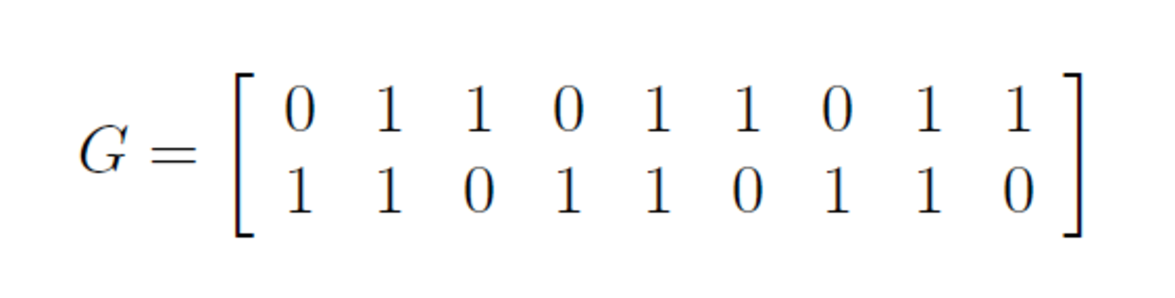
\includegraphics[width=6
%cm]{Fig1}
%%\caption{Generator matrix.}
%\end{figure}
%%\end{itemize}
%\item Determine the parity check matrix, and indicate the values assumed by the "sindrome" associated to a possible single bit error, a possible two bits error, and a possible 3 bits error. How many different sindromes are possible ?
\item 
\begin{itemize}
\item A block code is characterized by the Generator matrix given in Figure. Determine the possible codewords. Is this a cyclic code ? What is the generator polinomial ? What is the minimum distance ? 
\begin{figure}[ht] \centering
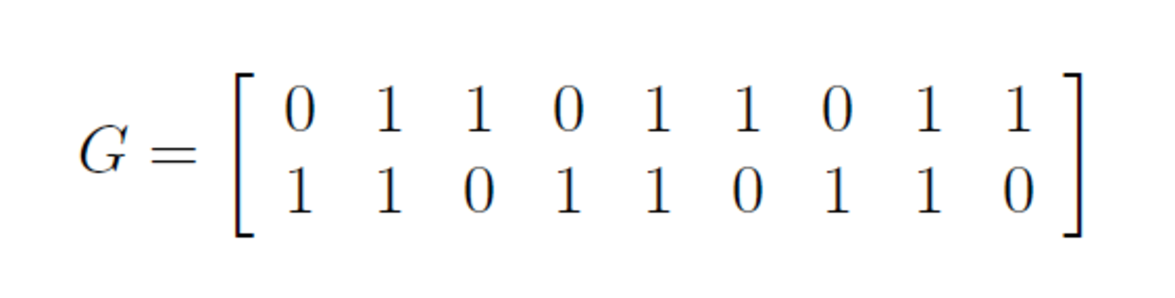
\includegraphics[width=7cm]{Fig1}
\end{figure}
\item A (7,4) cyclic linear block code is described by the generator polinomial $g(D)=D^3+D^2+1$. Indicate the values assumed by the "sindrome" associated to a possible single bit error, a possible two bits error, a possible three bits error. In case of 2 errors, how many different sindromes are possible ?
%\item Consider the Hamming code with $N=127$. Determine the error probability in case of both hard (use the more precise estimation) and soft decoding.
\item Consider the Hamming code with $N=127$. Determine the number of possible codewords, the error probability in case of both hard (use the more precise estimation) and soft decoding, and the minimum bandwidth required to transmit 10 Mbit/sec.
%\item Consider a block code with $N=48$, $K=24$, $d=12$. Determine the number of possible codewords, the probability of error (hard decision,  using the more precise approximation), and the minimum bandwidth required to transmit 10 Mbit/sec.\\
\end{itemize}
%\end{enumerate}
%\begin{enumerate}
%\item 
%\begin{itemize}
%\item A (7,4) cyclic linear block code is described by the generator polinomial $g(D)=D^3+D^2+1$. Indicate the possible code-words. Determine the generator matrix of this code, in its systematic shape.
%\item Indicate the values assumed by the "sindrome" associated to a possible single bit error, a possible two bits error, a possible three bits error.
%\item What is the probability of error in case of hard and soft decision ?
%\item What is the  minimum required bandwidth (in case of binary modulation) if the information bit-rate is equal to $1$ Mbit/s.
%\begin{itemize}
%\item Consider the Hamming code with $N=127$. Determine the error probability in case of both hard (use the more precise estimation) and soft decoding.
%\end{itemize}
%\item A block code is described by the parity check matrix indicated in Fig. 1. 
%\begin{itemize}
%\item Indicate the possible code-words. Is this a cyclic code ? 
%\item Indicate the possible values assumed by the "sindrome" associated to any possible single bit error.
%%\item What is the probability of error in case of hard and soft decision ?
%\item What is the  minimum required bandwidth (in case of binary modulation) if the information bit-rate is equal to $1$ Mbit/s.
%\end{itemize}
%%Indicate the possible code-words. Is this a systematic code ? Is this a cyclic code ? What is the minimum distance of this code ? %%What is the Parity Check Matrix ?
%\begin{figure}[ht] \centering
%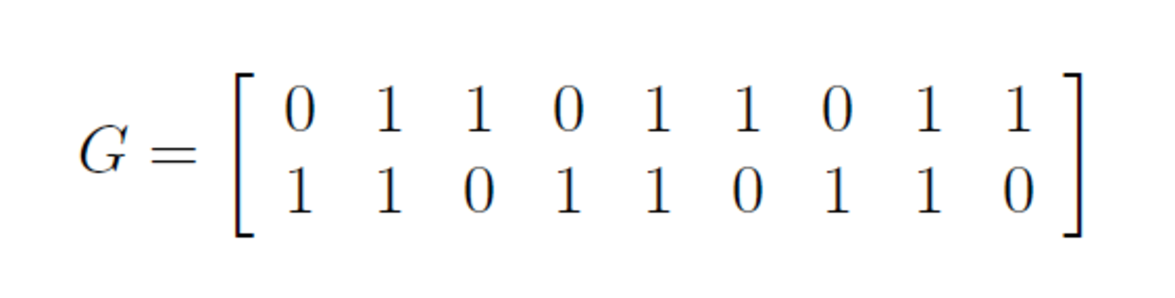
\includegraphics[width=6 cm]{Fig1.pdf}
%%{\caption{Sistema in esame.}}
%\end{figure}
%\item Consider the Hamming code with $N=127$. Determine the error probability in case of both hard (use the more precise estimation) and soft decoding.
%\item 
%Consider a block codes with $N=48$, $K=24$, $d_{min}=12$. Determine the number of possible code-words, the performance (in case of hard decision), and the  minimum required bandwidth (in case of binary modulation) if the bit-rate is equal to $100$ Mbit/s.
%\item 
%A block code is described by the parity check matrix indicated in Fig. 1.
%\begin{figure}[ht] \centering
%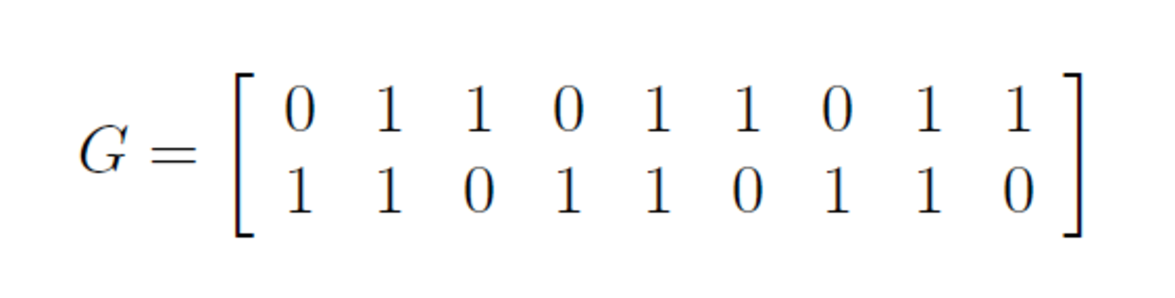
\includegraphics[width=5 cm]{Fig1}
%{\caption{Sistema in esame.}}
%\end{figure}
%\begin{itemize}
%\item Indicate the possible code-words.
%\item What is the probability of error in case of hard and soft decision ?
%\item What is the  minimum required bandwidth (in case of binary modulation) if the information bit-rate is equal to $10$ Mbit/s.
%\end{itemize}
%\item
%Design a (6, 2) cyclic code by choosing the longest possible generator polynomial\footnote{Hint: $D^6+1=(D+1)^3 \cdot (D+1)^3=(D+1) \cdot (D+1) \cdot (D^2+D+1) \cdot (D^2+D+1)$.}. 
%Determine the generator matrix G (in the systematic form) for this code and find all the possible codewords. How many errors can be corrected or detected by this code ? 
%\item A systematic block code is described by the parity check matrix H indicated in Fig. 1. Determine and draw the generator matrix of this code. Indicate the possible code-words. Is this a cyclic code ? 
%What is the probability of error in case of hard and soft decision ?
%\begin{figure}[ht] \centering
%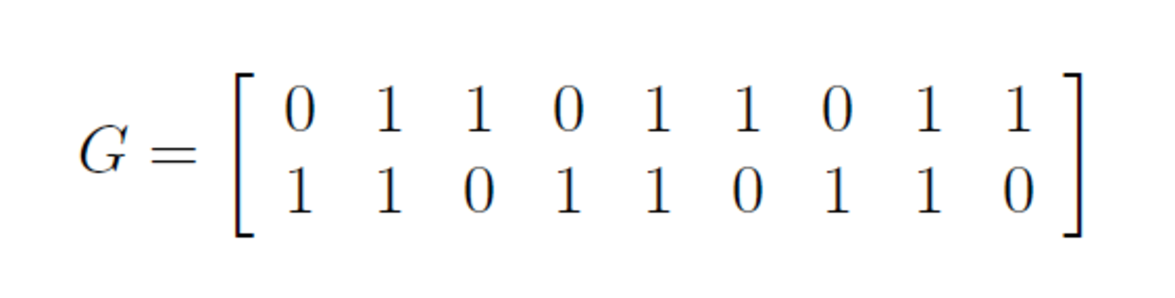
\includegraphics[width=5 cm]{Fig1}
%{\caption{Sistema in esame.}}
%\end{figure}
%\item What is the  minimum required bandwidth (in case of binary modulation) if the information bit-rate is equal to $10$ Mbit/s.
%\item Consider the Hamming code with $N=127$. Determine the error probability in case of both hard (use the more precise estimation) and soft decoding.
%\item A block code with $N = 7$ is characterized by the generator polynomial: $g(D) = (D+1)(D^3 +D+1)$. Determine the minimum distance of this code. Is this code a cyclic code ?
%\end{itemize}
%\item Consider the BCH code of length $N = 31$ and generator polynomial (in octal description)
%$107657$. In this code there is 1 word composed by all zeros, 155 words with 7 ones, 465 with 8 ones, 5208 with 11 ones, ...
%\begin{itemize}
%\item What is the generator polynomial of this code (g(D)= ...) ? Determine the number of possible codewords, and the probability of error (in case of hard and soft decision).
%\end{itemize}
%\end{itemize}

\item 

Consider the linear block code of length $N = 31$ and generator polynomial (in octal description)
$107657$. In this code there is 1 word composed by all zeros, 155 words with 7 ones, 465 with 8 ones, 5208 with 11 ones, ...

\begin{itemize} 
\item 
What is the generator polynomial of this code (g(D)= ...) ? Determine the number of possible codewords, and the probability of error (in case of hard and soft decision, using the more precise estimation).

\item The code is now extended adding a final parity check bit (imposing an EVEN number of "1").
%\begin{itemize}
%\item What is the generator polynomial of this code (g(D)= ...) ? Determine the number of possible codewords, and the probability of error (in case of hard and soft decision).
Determine the new probability of error (in case of hard and soft decision, using the more precise estimation).

\item Consider the following possible codewords (of the extended code).
\begin{itemize} 
\Large{
\item 
$00000000000001000111110101111001$ is a valid codeword ?
\item
$00000000000001111010111110001001$ is a valid codeword ?
}
\end{itemize}
%}
%\end{itemize}
\end{itemize}

%\item  %(b) What is the  minimum required bandwidth (in case of binary modulation) if the information bit-rate is equal to $1$ Mbit/s.
%Design a (6, 2) cyclic code by choosing the shortest possible generator polynomial\footnote{Hint: $D^6+1=(D+1)^3 \cdot (D+1)^3=(D+1) \cdot (D+1) \cdot (D^2+D+1) \cdot (D^2+D+1)$.}. 
%Determine the generator matrix G (in the systematic form) for this code and find all the possible codewords. How many errors can be corrected or detected by this code ? 

%\item A block code with $N = 7$ is characterized by the generator polynomial: $g(D) = (D+1)(D^3 +D+1)$. %Determine the minimum distance of this code. 
%s this code a cyclic code ?


%\item Consider the following possible codewords.
%\large{
%\begin{itemize} \item (c) 00000000000001000111110101111001 is a valid codeword ? \item (d) 00000000000001111010111110001001 is a valid codeword ?
%}
%\end{itemize}
%\end{itemize}

%\item Consider now a Hamming code with $N=127$. Determine the error probability in case of both hard (use the more precise estimation) and soft decoding.
%\item Consider now a block code with: $N=48$, $K=24$, $d=12$. Determine the number of possible codewords, the probability of error (in case of hard and soft decision) and the minimum required bandwidth if the transmitted information bit-rate is $100$ Mbit/s.

%\newpage .
%\newpage

%\item 
%Consider a block codes with $N=48$, $K=24$, $d_{min}=12$. 
%\begin{itemize}
%\item Determine the number of possible code-words, the performance (in case of hard decision), and the  minimum required bandwidth (in case of binary modulation) if the bit-rate is equal to $100$ Mbit/s.
%\end{itemize}
%Consider a Hamming code with $N=127$.
%\begin{itemize}
%\item Determine the error probability in case of hard and soft decoding.
%\end{enumerate}
%\newpage

\item
%Consider a convolutional code with $R=1/3$, and octal generators $(1, 2, 3)$. 
%Determine and draw the tree, trellis, and the state diagrams of the code. 
\begin{itemize}
\item  Consider a convolutional code with $R=1/3$, and octal generators $(1,2,3)$. Determine and draw the trellis and tree diagram of the code. 
%\item The received sequence (hard decision) is equal to: $000, 110, 010, 110, 011, 110, 101, 011, 000$. Determine, applying the Viterbi algorithm, the maximTum likelihood transmitted sequence (related to information bits).
\item Determine the bit-error probability, considering at least 3 non zero terms in the union bound.
\item Determine the code word associated to the information sequence: $010101100$, and the minimal bandwidth required in case of an information bit-rate equal to 1 Mbit/sec.\\
\end{itemize}

\end{enumerate}
%\newpage 
%\newpage

%\item Consider a convolutional code with $R=1/2$, and octal generators $(5, 7)$. 
%\begin{itemize}
%\item Draw the tree diagram of the code. 
%\item Determine the code word associated to the information sequence $010101100$, and the minimum bandwidth required in case of an information bit-rate equal to 100 Mbit/sec.
%%\item Determine and draw the trellis diagram of the code. 
%\item The received sequence (hard decision) is equal to: $000, 110, 010, 110, 011, 110, 101, 011, 000$. Determine, applying the Viterbi algorithm, the maximum likelihood transmitted sequence (related to information bits).
%\item Determine the bit-error probability (considering at least 3 error events (i.e., minimum distance, the next, the next) in the union bound).
%\end{itemize}

%\newpage
{\bf Part2 (Theoretical Description)} \\
\begin{enumerate}
\item Optimal receiver
\begin{itemize}
\item Define and describe the likelihood function related to the optimal receiver in case of AWGN noise.
\item Define and describe the equations related to the concept of "complex envelope". %Indicate the use of this concept in case of pass-band signals.
%\item Define and describe the equations related to the concept of signal vector spaces.
\end{itemize}

\item OFDM
\begin{itemize}
%\item[D11.]  Descrivere in dettaglio lo schema a blocchi del sistema di trasmissione e di ricezione nel caso di modulazione OFDM, 
%\item[D11.]  Indicare come, partendo dall'espressione analitica del segnale OFDM, si possa ricavare lo schema a blocchi dettagliato del modulatore e del demodulatore.
\item Describe the analytical expression of an OFDM symbol and the block diagram of an OFDM encoder.
%\item Describe the block diagram of an OFDM encoder.
\item Describe the channel equalization procedure performed in the OFDM modulation systems.
%\item Discuss about the main advantages and problems of the OFDM modulation systems.
%\item Describe in some detail the channel equalization procedure used in the OFDM modulation systems (focusing also on the cyclic prefix and pilot carriers).
%, indicating the role of the cyclic prefix and of the pilot carriers.
%\item[D12.]  Descrivere la tecnica di equalizzazione adottata nei sistemi OFDM, spiegando precisamente il significato del prefisso circolare e delle portanti pilota.
%\newpage
%\item[D13.]  Descrivere i principali vantaggi e svantaggi della modulazione OFDM.

%\newpage .
%\newpage

%\item[D21.]  Descrivere in dettaglio lo schema a blocchi del sistema di trasmissione e di ricezione nel caso di modulazione a spettro espanso DSSS.
%\item[D21.]  Descrivere il principio di funzionamento della modulazione a spettro espanso DSSS, indicando in quali contesti questa garantisce dei vantaggi rispetto alle modulazioni tradizionali.
%\newpage
\end{itemize}

\item DSSS
\begin{itemize}
%\item Define and describe the basic properties of the m-sequences. Why are this seq. used in the DSSS modulation ?
\item Describe why and when a DSSS modulation system is robust against multi-path fading.
%\item Describe the basic ideas used in the CDMA systems, giving also an idea about its performance.
\item Describe the basic idea of the Rake Receiver, indicating also why this is working properly in the case of DSSS modulation.
%\newpage
%\item[D23.]  Nel contesto del CDMA, descrivere il principio di funzionamento del Rake Receiver, indicando perch\'e questo pu\`o funzionare bene nel caso in cui la modulazione utilizzata sia del tipo DSSS.
%\newpage
%\newpage .
%\newpage
\end{itemize}
\item CPM
\begin{itemize}
%\item Describe the analytical expression of the modulated signal in case of MSK modulation, and its phase tree.
%\item Draw the phase-tree in the case of MSK modulation.
\item Describe the analytical expression of the likelihood function that should be maximized by the optimal receiver in the case of MSK modulation.
%\item Describe the major strategies used to simplify the CPM receivers.
%\item Describe the basic parameters of the MSK modulation system.
%\item Describe the major strategies used to simplify the CPM receivers.
%\item[D31.]  Descrivere in dettaglio la modulazione MSK.
%\item[D31.]  Descrivere la modulazione MSK, indicando l'espressione analitica della funzione di verosimiglianza che deve massimizzare il ricevitore ottimo.
%\newpage
%\item[D32.]  Nel caso di modulazione MSK, indicare come si possa calcolare la distanza tra due possibili segnali trasmessi. Che traiettorie di fase portano alla distanza minima ? Quanto vale la distanza minima in questi casi ?
%\newpage
%\item[D33.]  Descrivere (anche analiticamente) la tecnica utilizzata per stimare lo spettro di potenza di una modulazione CPM (commentare i vari passaggi effettuati, le ipotesi assunte a priori ed il loro impatto durante il procedimento di stima).
\end{itemize}

\item Turbo-LDPC Codes
\begin{itemize}
%\item Describe the block diagram of a turbo encoder / decoder.
%\item Describe the curves that represents the performance (P(E) as a function of Eb/No) of a turbo code, indicating the role of the iterations, and the role of the inter-leaver.
\item Describe the basic idea of the bit-flipping algorithm for the decoding of an LDCP code.
%\item Describe the basic idea of the Tanner graphs, using a simple example.
\item Describe the basic idea and the motivation of the EXIT charts.
\end{itemize}
%\newpage .
%\newpage


\end{enumerate}

%\newpage .
%\newpage


%\end{enumerate}
%}
\end{document}
